\documentclass{article}
\usepackage{listings}
\usepackage{amsmath}
\usepackage{blindtext}
\usepackage{amssymb}
\usepackage{graphicx}
\usepackage[a4paper, margin=1in]{geometry}

\lstset{
	numbers=left,                                        
 	frame=none,                                         
	tabsize=4,
	keywordstyle=\color{blue},
}
\title{Proposal for Master Minds}
\author{Xinhao Su \and David Xu}
\begin{document}
\maketitle
\section{Introduction}
Master Mind is a code breaking game that was invented in 1970 by Mordecai Meirowitz. 
It resembles the earlier paper and pencil game 
called Bulls and Cows that may date back a century. 
The gameplay of Master Mind is straightforward:
\begin{enumerate}
	\item The codemaker picks 4 pegs (which can each be one of 6 different colors), and places them in order as the code. (Note that the code can have repeated colors, e.g. red red blue blue)
	\item The codebreaker needs to guess both the color and the order of the code within 8 turns. 
	\item At each turn, the codemaker provides feedback by placing 0 to 4 pegs in response to a guess.
	A black peg indicates that one of the pegs in the guess is correct in both color and order. 
	A white peg indicates that one of the pegs in the guess is correct in color but not order. 
	\item The game is terminated when the codebreaker's guess is correct or 8 incorrect guesses have been made.
\end{enumerate}
\begin{figure}[h]
	\centering
	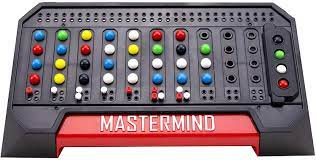
\includegraphics{mm.jpeg}
\end{figure}
Since we will use parallelism to find the solution, our project will be called \textit{Master Minds}.


\pagebreak
\section{Algorithm}

The Master Mind game can be rephrased as The Mastermind Problem: 
Given a set of guesses and the feedback for each guess (number of colored and white pegs), is there at least one code that generates those exact feedback reponses?
It is interesting to note that this problem is in effect a multi-dimensional search problem.
The Mastermind Problem has been proven to be NP-Complete\footnote{Stuckman, J., \& Zhang, G. Q. (2005). Mastermind is NP-complete. \textit{arXiv preprint cs/0512049}.}.

\paragraph[]{Our project will use Donald Knuth's Five-Guess Algorithm\footnote{Knuth, D. E. (1976). The computer as master mind. \textit{Journal of Recreational Mathematics, 9}(1), 1-6.} to break the code:}

\begin{enumerate}
	\item Generate the set of possible codes, denoted as $S$. E.g., $S= \{ 6^4=1296 \ codes\}$
	\item Start with an initial guess (initial guess can be hardcoded or randomly selected from $S$) 
	\item Play the guess and get response from codemaker
	\item If the feedback is all black, we have found the code.
	\item Otherwise, remove all the codes that would not produce the most recent response from $S$. For example, if our guess had two blues and the response is only one white peg, then we know the true code cannot have two blues.
	\item For the next guess, select a code (not necessarily in $S$) which minimizes the maximum possible number of remaining codes in $S$ across all possible true codes.
	\item Repeat from Step 3.
\end{enumerate}

\section{Testing Plan}
Since the Mastermind game has many variations, we intend to test our project on all or some of the following variations:
\begin{enumerate}
	\item Mastermind - 6 colors, guessing 4 pegs 
	\item New Mastermind - 8 colors, guessing 4 pegs 
	\item Word Mastermind - 26 letter, guessing 4 letters
	\item Grand Mastermind - 5 colors with 5 shapes, guessing 4 pegs 
	\item Crazy Mastermind - 12 colors, guessing 4 pegs 

\end{enumerate}
Our project could also be used to analyze which codewords minimize the maximum or average number of guesses required based on which initial guess is used for each of these variations.

\section{Opportunities for Parallelization}
\begin{enumerate}
	\item The execution of the algorithm with different initial guesses is embarrassingly parallelizable.
	\item In the process of selecting the next guess, the calculation of the worst-case (maximum possible) number of remaining codes for any given guess can be parallelized.
	\item If we desire to play multiple variations of the game at the same time, such gameplay can also be parallelized.
\end{enumerate}
\end{document}
